\chapter{Kodeeksempler}\label{ch:appendix-kodeeksempler}

\section{Enumerate / Itemize}
Enumerate bruges til at lave en liste, fx med tal, bogstaver eller romertal. Itemize bruges til bullets.

\begin{lstlisting}[language=Tex, caption=Her vises enumerate med forskellige formatering af tallet]
 \begin{enumerate}[label=\textbf{\arabic*: }]
    \item This is the first item
    \item This is the second item
\end{enumerate}

 \begin{enumerate}[label=\textit{\roman*.  }]   % roman = i ii iii, Roman = I II III
    \item This is the third item
    \item This is the fourth item
\end{enumerate}

 \begin{enumerate}[label=\Alph*) ]    % alph = a b c, Alph = A B C
    \item This is the fifth item
    \item This is the sixth item
\end{enumerate}

\begin{itemize}[itemsep=1pt]    % itemsep = afstand ml punkter
    \item This is the final item
\end{itemize}
\end{lstlisting}

\subsection{Eksempel:}

 \begin{enumerate}[label=\textbf{\arabic*: }]
    \item This is the first item
    \item This is the second item
\end{enumerate}

 \begin{enumerate}[label=\textit{\roman*.  }]   % roman = i ii iii, Roman = I II III
    \item This is the third item
    \item This is the fourth item
\end{enumerate}

 \begin{enumerate}[label=\Alph*) ]    % alph = a b c, Alph = A B C
    \item This is the fifth item
    \item This is the sixth item
\end{enumerate}

\begin{itemize}[itemsep=1pt]    % itemsep = afstand ml punkter
    \item This is the final item
\end{itemize}

\pagebreak

\section{wrapTable / wrapFigure}
Wraptable/figure bruges til at få teksten til at gå rundt om billedet. Ligesom i Word, hvor man kan vælge at wrape teksten rundt om et billede.
De to environments har samme formatering, men wrapTable gør så elementet referes som tabel, hvis man bruger en label, og wrapFigure refererer til . 

\begin{lstlisting}[language=Tex, caption=Her vises brug af wrapTable]
    \lipsum[4]    % Dummytekst
    \begin{wrapfigure}{r}{8cm} % {r} betyder hoejrejusteret, {8cm} er bredden af containeren
    
        \centering  % Centrerer billedet i wrap-containeren
        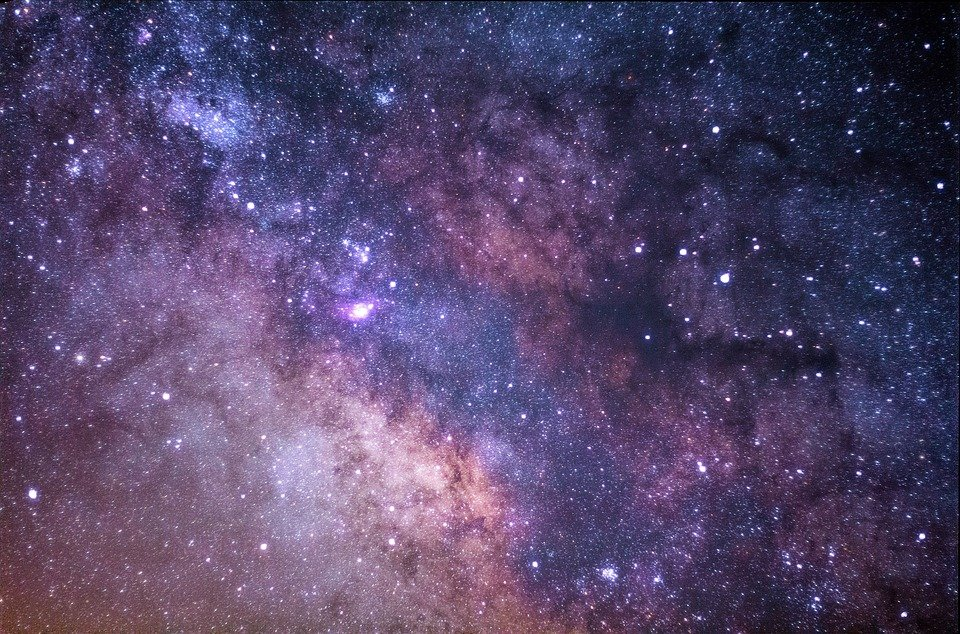
\includegraphics[width=0.95\linewidth]{media/AAUgraphics/frontpageImage.jpg} % width er billedets bredde, linewidth refererer til bredden af wrap-containeren
        
        \caption{SPAAAAAAAAAAAAAAAAACEEEEEEEE!}
        \label{fig:wraptable}
        
    \end{wrapfigure}
    
    \lipsum[4-5]    % Dummytekst
\end{lstlisting}

\subsection{Eksempel:}
\lipsum[4]    % Dummytekst
\begin{wrapfigure}{r}{8cm} % {r} betyder højrejusteret, {8cm} er bredden af containeren
    \centering
    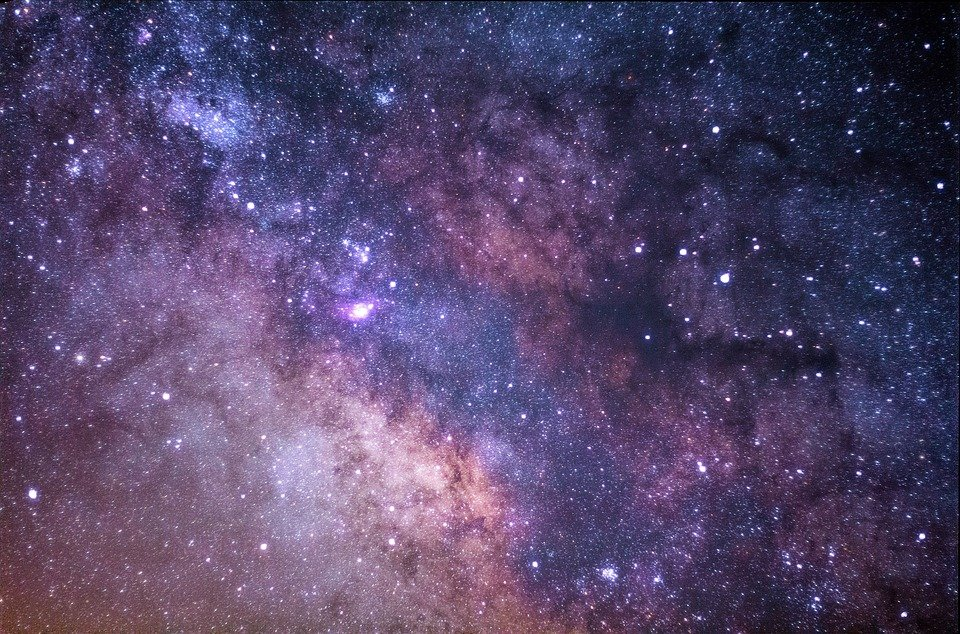
\includegraphics[width=0.95\linewidth]{media/AAUgraphics/frontpageImage.jpg} 
    % width er billedets bredde, linewidth refererer til bredden af containeren, så 0.95*linewidth giver lidt margin om billedet. 
    \caption{SPAAAAAAAAAAAAAAAAACEEEEEEEE!}
    \label{fig:wraptable}
\end{wrapfigure}
\vspace{-0cm} % nogle gange er der whitespace efter figuren. Det fjernes med fx -1cm vspace
\lipsum[4-5]    % Dummytekst

\pagebreak

\section{Minipages - To billeder ved siden af hinanden}
Hvis vi gerne vil have to billeder ved siden af hinanden kan vi dele siden op i to minipages.

\begin{lstlisting}[language=Tex, caption=Her vises brug af wrapTable]
\lipsum[64]
\par
\vspace{1cm}
\noindent % vigtigt at have med
\begin{minipage}{0.5\textwidth} % hver minipage er 0.5 sidebredde i bred
    \centering
    
\includegraphics[width=0.8\linewidth]{media/AAUgraphics/aau_logo_circle_en.pdf} 
    \captionof{figure}{AAUs cirkel-logo paa engelsk} % NB: captionof ikke caption
    \label{fig:aauLogoEN}
\end{minipage}%
%
\begin{minipage}{0.5\textwidth}
    \centering
    
\includegraphics[width=0.8\linewidth]{media/AAUgraphics/aau_logo_circle_da.pdf} 
    \captionof{figure}{AAUs cirkel-logo paa engelsk} % NB: captionof ikke caption
    \label{fig:aauLogoDA}
\end{minipage}
\end{lstlisting}

\noindent
Note: Vi bruger kommandoen captionof{figure}{caption skrives her} i stedet for almindeligvist at bruge caption{caption skrives her}, da vi ikke er inde i et korrekt "float environment". Det er fordi vi er inde i et minipage-environment som ikke definerer om det er en figur eller en tabel der er tale om.

\subsection{Eksempel:}
\lipsum[64]
\par
\vspace{1cm}
\noindent % vigtigt at have med
\begin{minipage}{0.5\textwidth} % hver minipage er 0.5 sidebredde i bred
    \centering
    
\includegraphics[width=0.65\linewidth]{media/AAUgraphics/aau_logo_circle_en.pdf} 
    \captionof{figure}{AAUs cirkel-logo på engelsk} % bemærk \captionof ikke \caption
    \label{fig:aauLogoEN}
\end{minipage}%
%
\begin{minipage}{0.5\textwidth}
    \centering
    
\includegraphics[width=0.65\linewidth]{media/AAUgraphics/aau_logo_circle_da.pdf} 
    \captionof{figure}{AAUs cirkel-logo på engelsk} % bemærk \captionof ikke \caption
    \label{fig:aauLogoDA}
\end{minipage}

